\chapter{Implementação do Sistema}

Nessa etapa efetuamos a implementação do sistema e colocamos ele em produção. Isso envolveu definir as versões específicas das tecnologias e frameworks que serão utilizados para o desenvolvimento da aplicação. Essas escolhas são fundamentais para garantir compatibilidade, segurança e aproveitamento das últimas funcionalidades disponíveis.

\section{Front-End Web Desktop}
\begin{itemize}
\item Agurdando infos
\end{itemize}

\section{Agente Desktop}

\begin{itemize}
\item Golang 1.18.1
\end{itemize}



\section{Back-end Versões e Frameworks}
\begin{itemize}
\item Esperando Infos
\end{itemize}
\subsection{Banco de dados}
\begin{itemize}
\item Supabase (Banco de dados Postgres na nuvem)
\end{itemize}
\subsection{Hospedagem}
\begin{itemize}
\item A definir
\end{itemize}


\section{Implementação}

\begin{figure} [H]
    \centering
    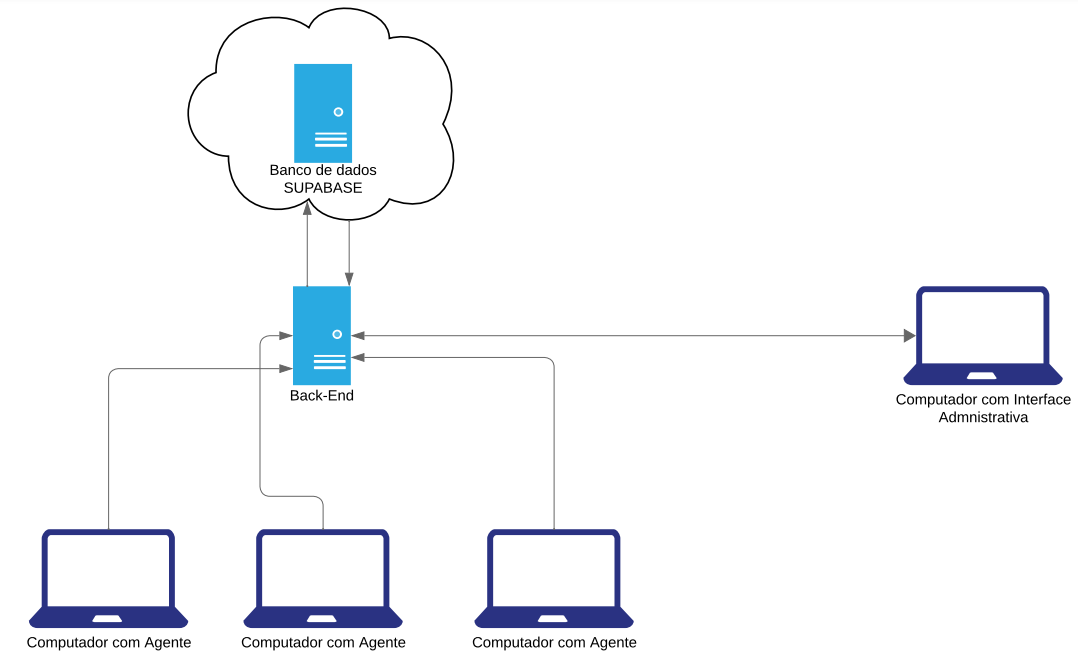
\includegraphics[width=1\linewidth]{figuras/INFRAIMPLE.png}
    \caption{Diagrama de implementação}
    \label{fig:diaimplementa}
\end{figure}
Na Figura \ref{fig:diaimplementa} Acima, pode-se observar como foi realizada a implementação com um back-end compartilhado para a interface de gerenciamento desktop e os agentes distribuídos. Para que o desenvolvimento de ambos os componentes ocorresse de maneira eficiente e integrada, foi necessário manter uma organização sólida entre o back-end e as funcionalidades específicas de cada parte do sistema.

\section{Geração de Dados Simulados}
Antes do início do desenvolvimento, as partes interessadas (Backend e Frontend e Agente) ajustaram previamente quais seriam os endpoints e as estruturas dos dados retornados pela API backend. Isso possibilitou a utilização de uma ferramenta chamada Mockaroo (https://www.mockaroo.com/), que serviu como um mock de dados e permitiu que as partes trabalhassem simultaneamente sem a dependência uma da outra.

Apenas no final do processo, as partes se juntaram para realizar uma parte da validação, garantindo que a conexão entre as partes não disparasse nenhum erro, independentemente do ambiente no qual o código estava sendo executado.

A outra parte da validação foi feita manualmente, com o acesso às telas buscando por caminhos diferentes para garantir que nenhum cenário fosse capaz de quebrar a aplicação.

\begin{figure}[H]
    \centering
    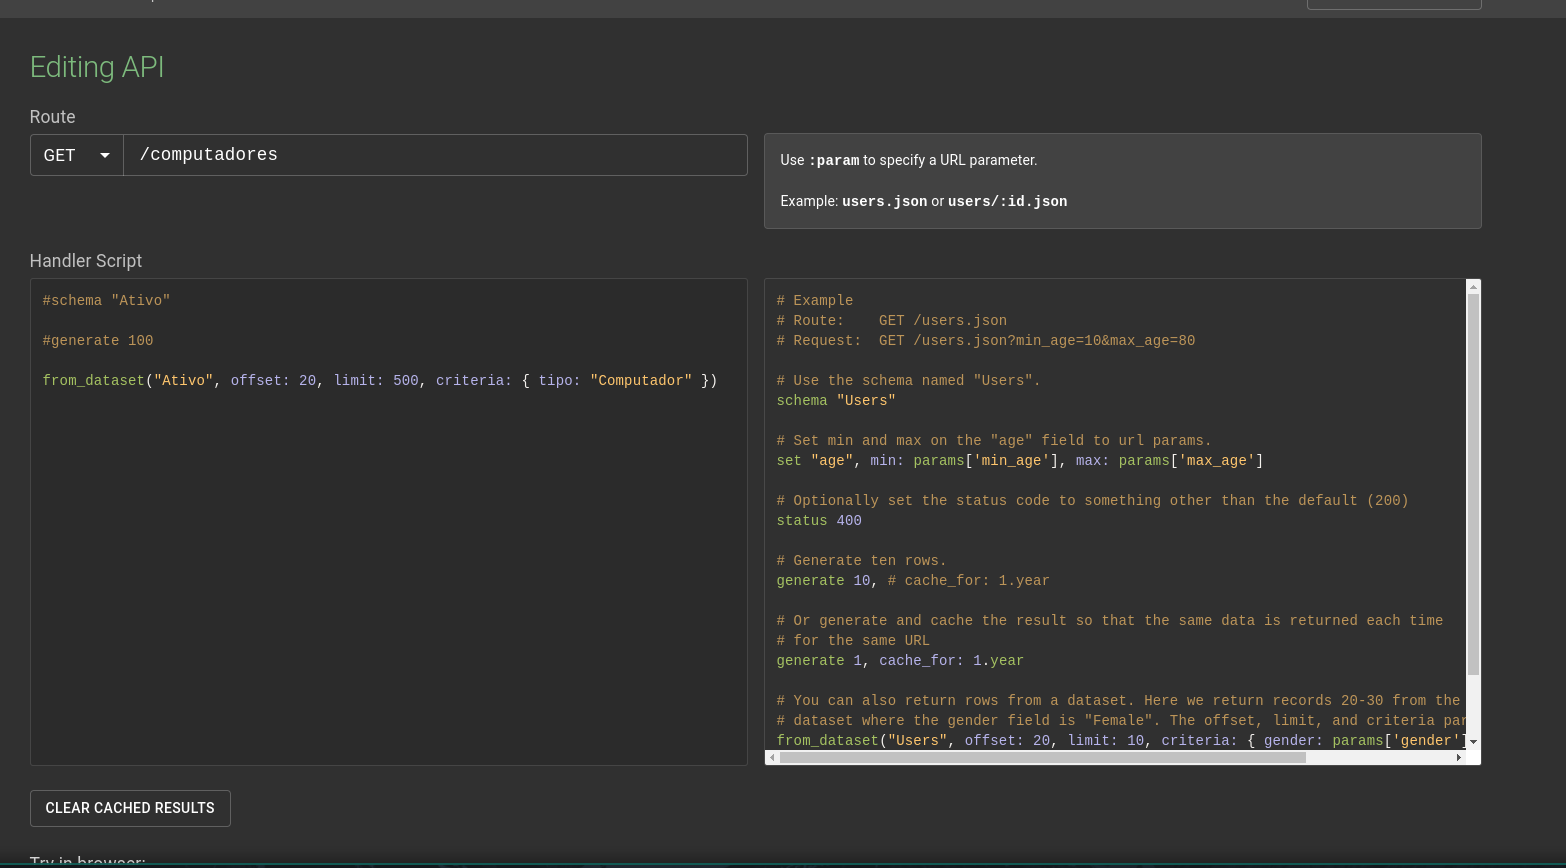
\includegraphics[width=0.6\linewidth]{figuras/apicomputador.png}
    \caption{Geração de requisições no mockaroo}
    \label{fig:enter-label}
\end{figure}

\begin{figure}[H]
    \centering
    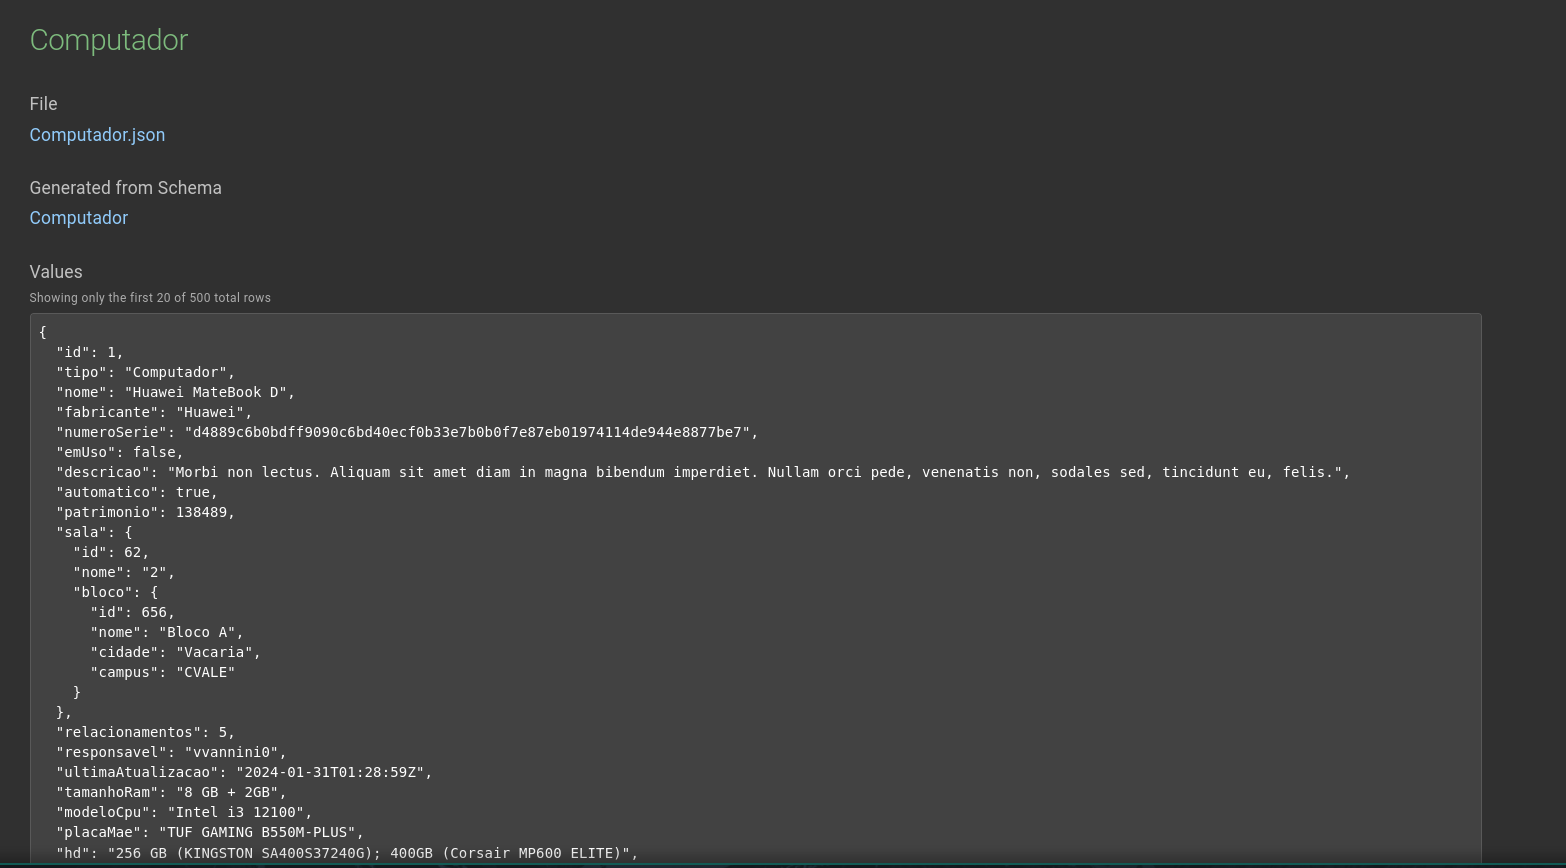
\includegraphics[width=0.6\linewidth]{figuras/mockcomputador.png}
    \caption{Exmplo de alguns formatos de dados}
    \label{fig:enter-label}
\end{figure}

Acreditamos que a utilização e organização com o Mockaroo foi essencial para que o desenvolvimento front-end e back-end e Agente pudesse ocorrer simultaneamente, sem que um dependesse do outro. O Mockaroo criou uma API com dados simulados, permitindo que o front-end realizasse testes e o back-end tivesse uma noção precisa de como deveria enviar os dados.

\section{Ferramentas para Utilização do Usuário}
\subsection{Interface Administrativa}
\begin{itemize}
\item Windows 10/11 e Linux
\end{itemize}
\subsection{Agente Desktop}
\begin{itemize}
\item Windows 10 /11 com o Powershell Atualizado
\end{itemize}


\section{Implementação Front-End Web}
Na criação da nossa aplicação web, nosso objetivo principal era exibir informações, com um foco significativo no design e na funcionalidade administrativa para adicionar e gerenciamento de conteúdo. Priorizamos especialmente a versão inicial para dispositivos móveis, garantindo exibições completas de todas as funcionalidades.



\subsection{Tela Principal}

\begin{figure}[H]
    \centering
    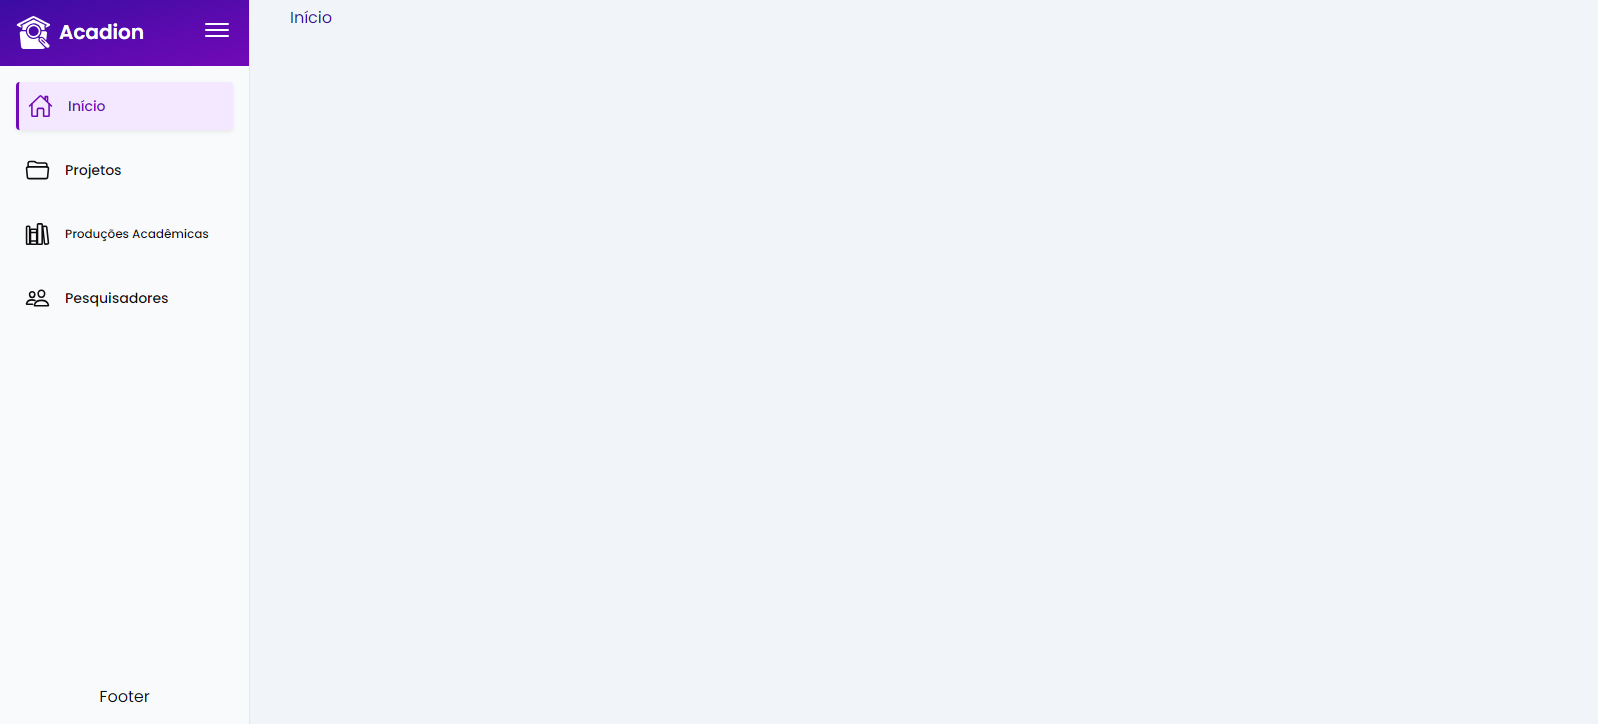
\includegraphics[width=1\linewidth]{figuras/SiteTelaPrincipal.png}
    \caption{Tela Início Web}
    \label{fig:enter-label}
\end{figure}
Optamos por focar nas funcionalidades principais, deixando propositalmente a implementação da tela inicial para um momento posterior.

\subsection{Tela Projetos}
\begin{figure}[H]
    \centering
    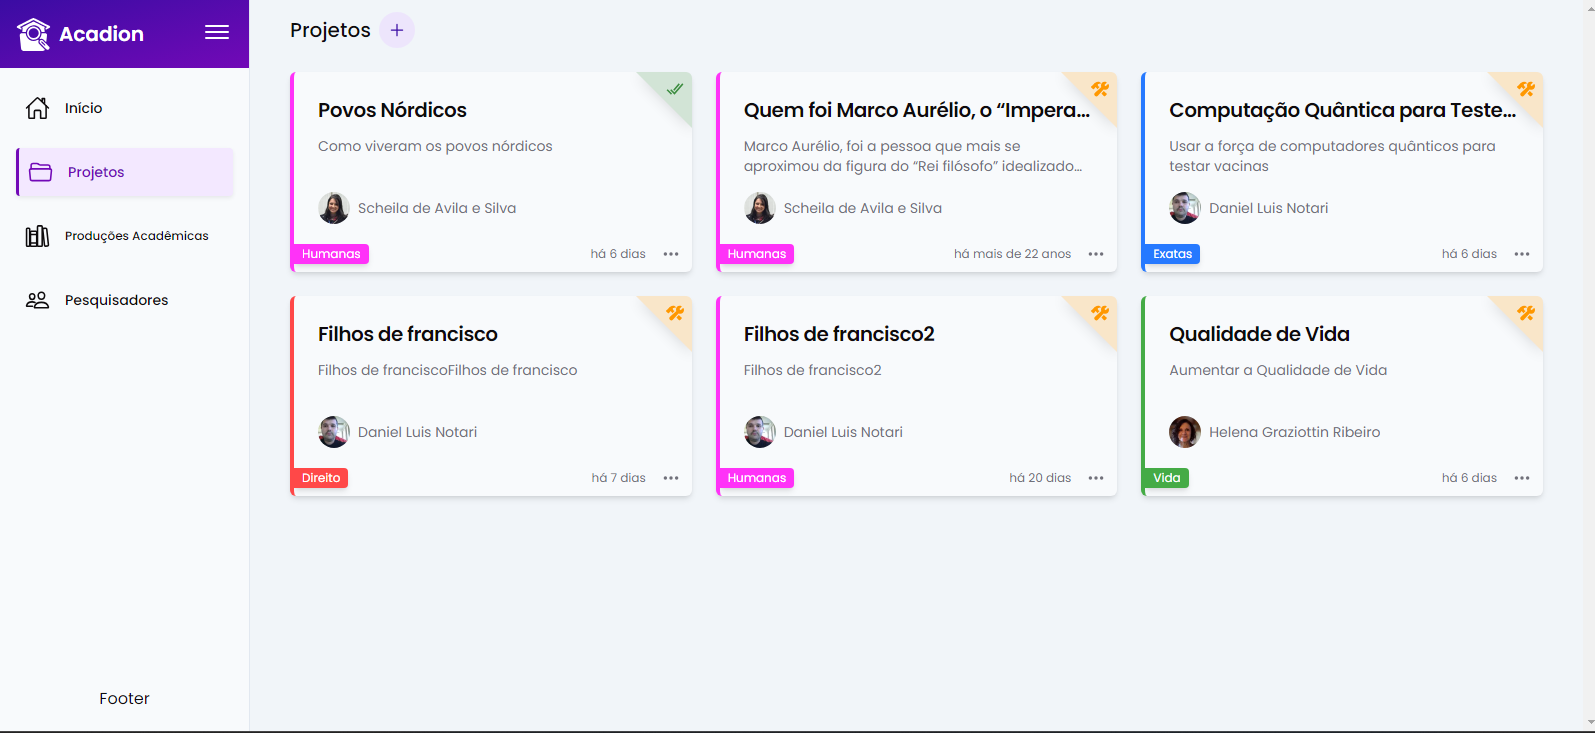
\includegraphics[width=1\linewidth]{figuras/TelaWebProjetos.png}
    \caption{Listagem dos projetos}
    \label{fig:projsweb}
\end{figure}
Nesta tela figura \ref{fig:projsweb}, são exibidos todos os projetos, mostrando o nome, um breve resumo e o coordenador de cada um. Além disso, é apresentada a área principal do projeto e seu status.

\begin{figure}[H]
    \centering
    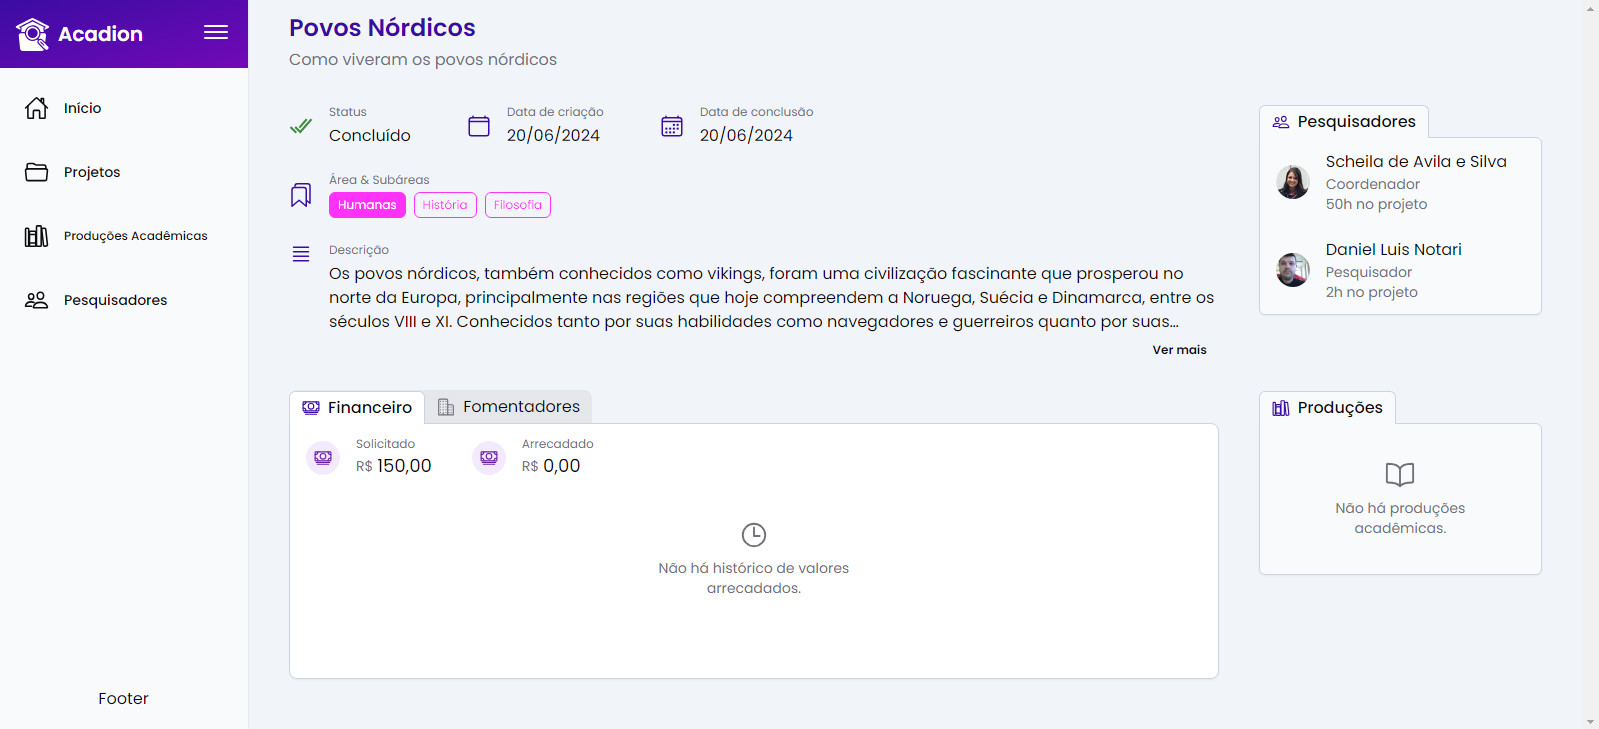
\includegraphics[width=1\linewidth]{figuras/DentroDeProjetos.png}
    \caption{Detalhes do projeto}
    \label{fig:detprojsweb}
\end{figure}
Nesta tela figura \ref{fig:detprojsweb}, são exibidos os detalhes do projeto selecionado, mostrando seu status, data de criação e conclusão. Também são apresentados todos os pesquisadores envolvidos, suas produções publicadas e a parte financeira, incluindo seus fomentadores.

\subsection{Adição de um Novo Projeto}
\begin{figure}[H]
    \centering
    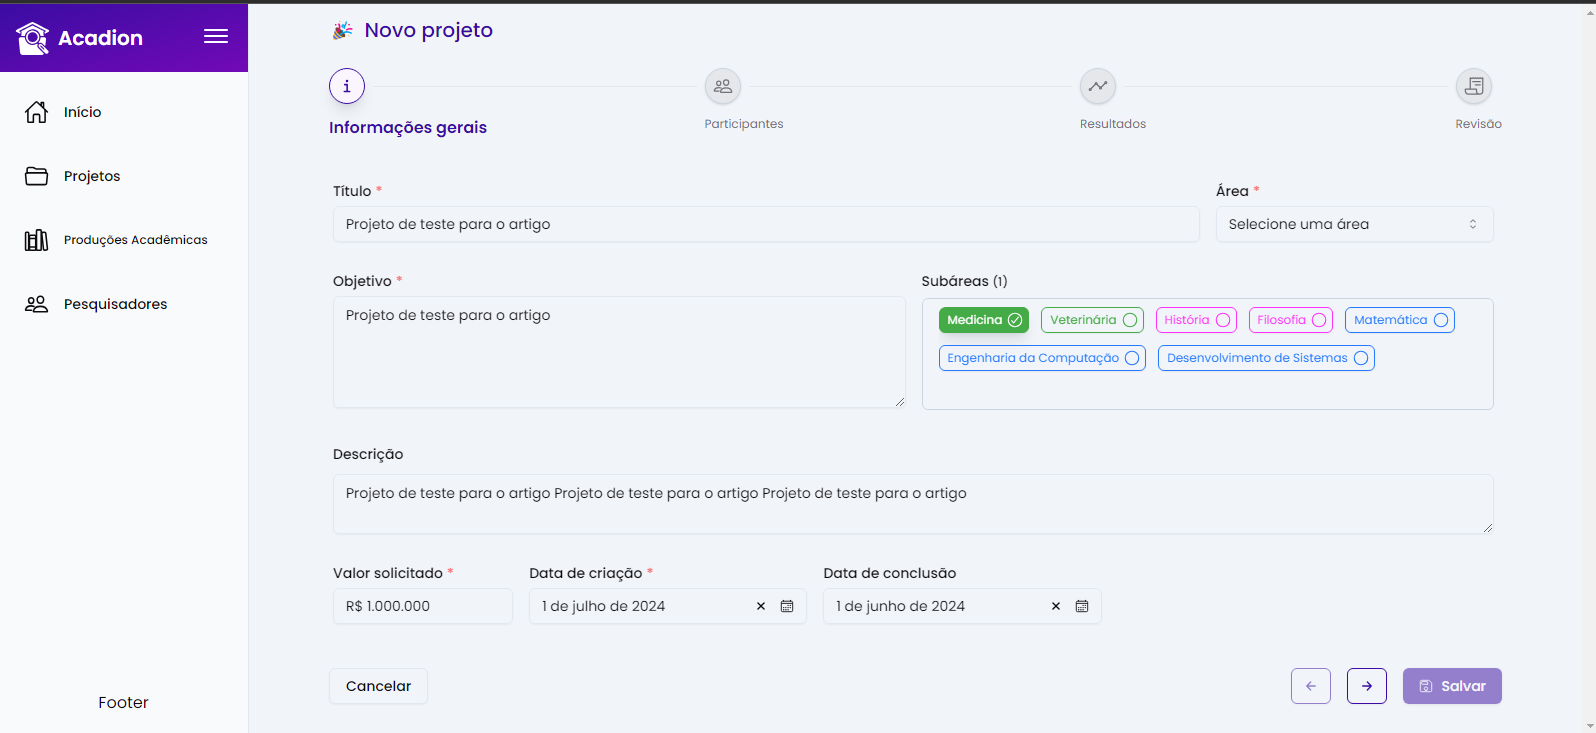
\includegraphics[width=1\linewidth]{figuras/NovoProjetoIG.png}
    \caption{Novo Projeto Informações gerais}
    \label{fig:addnewprojweb}
\end{figure}

\begin{figure}[H]
    \centering
    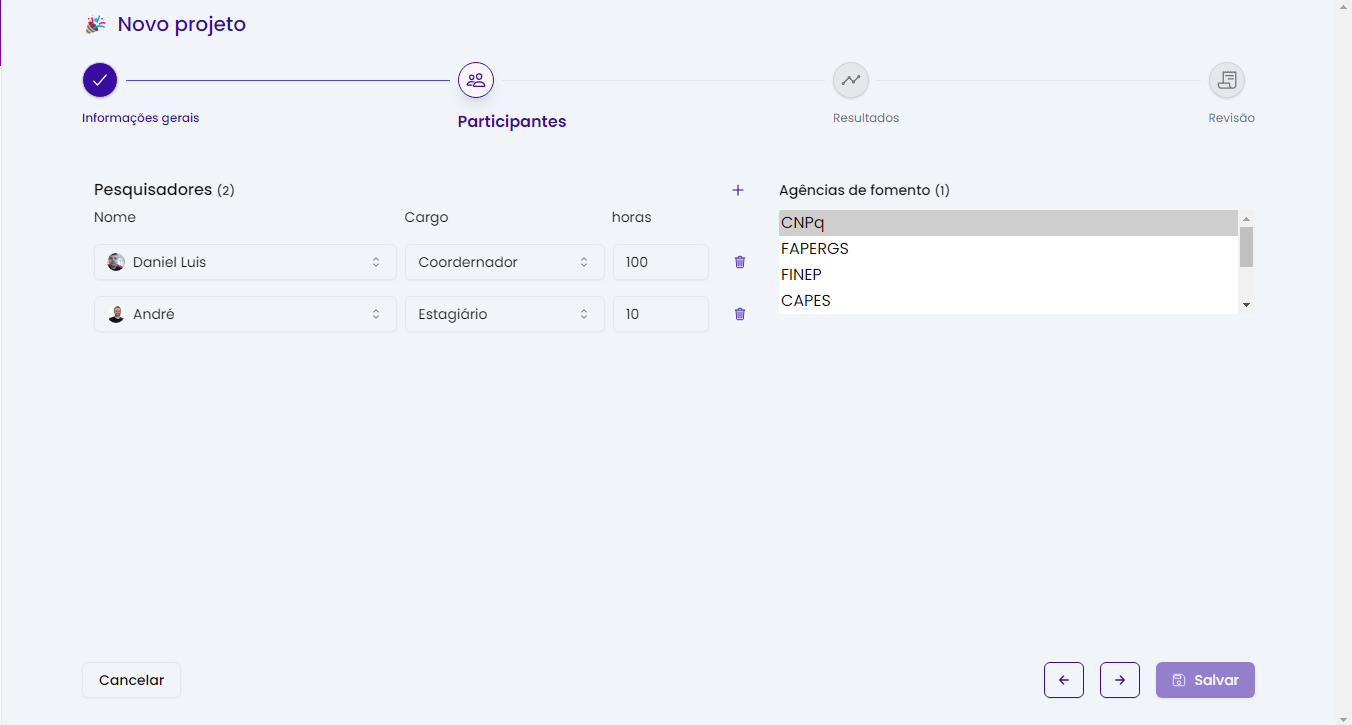
\includegraphics[width=1\linewidth]{figuras/NovoPorjetoParti.png}
    \caption{Novo Projeto Participantes}
    \label{fig:enter-label}
\end{figure}
\begin{figure}[H]
    \centering
    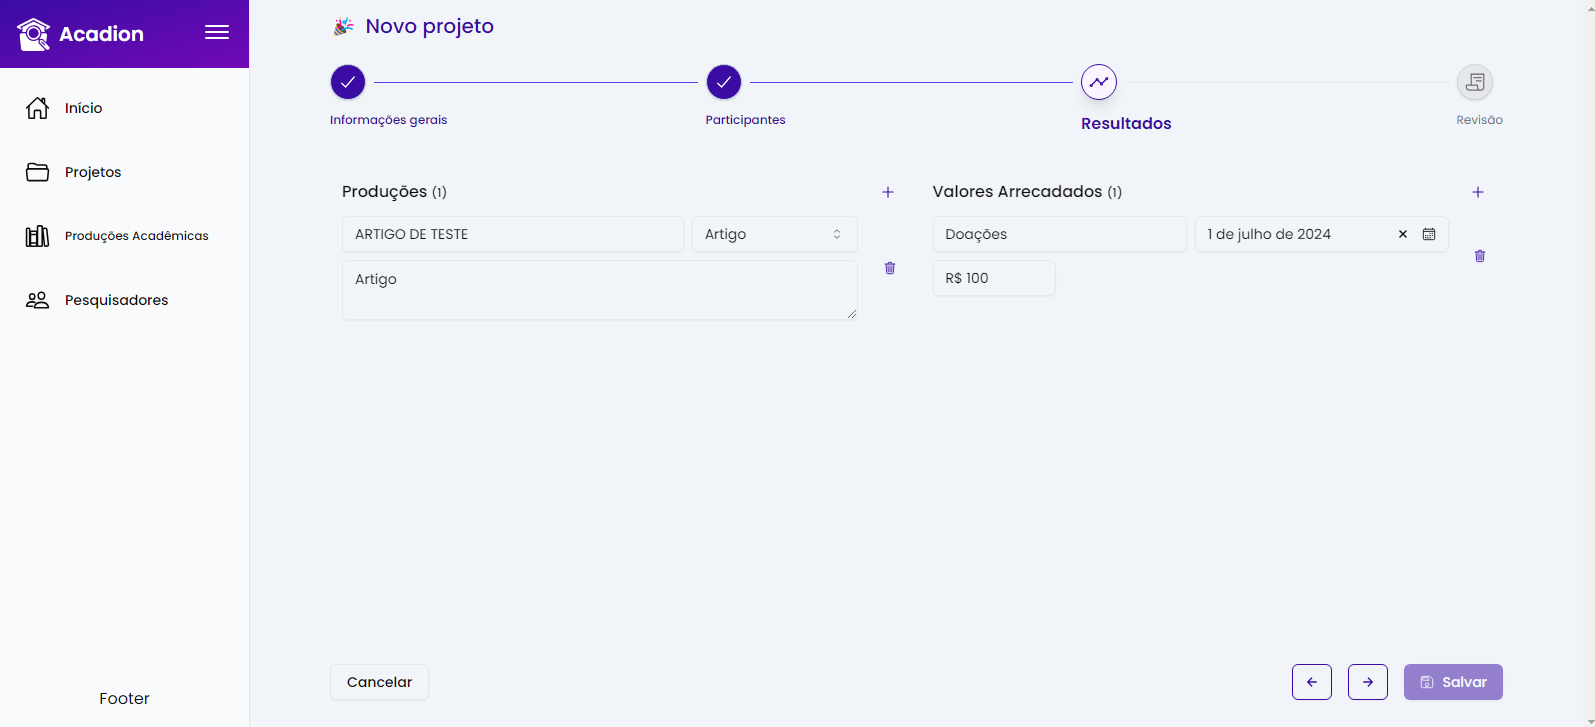
\includegraphics[width=1\linewidth]{figuras/NovoPorjetoResultados.png}
    \caption{Novo Projeto Resultados}
    \label{fig:enter-label}
\end{figure}

\begin{figure}[H]
    \centering
    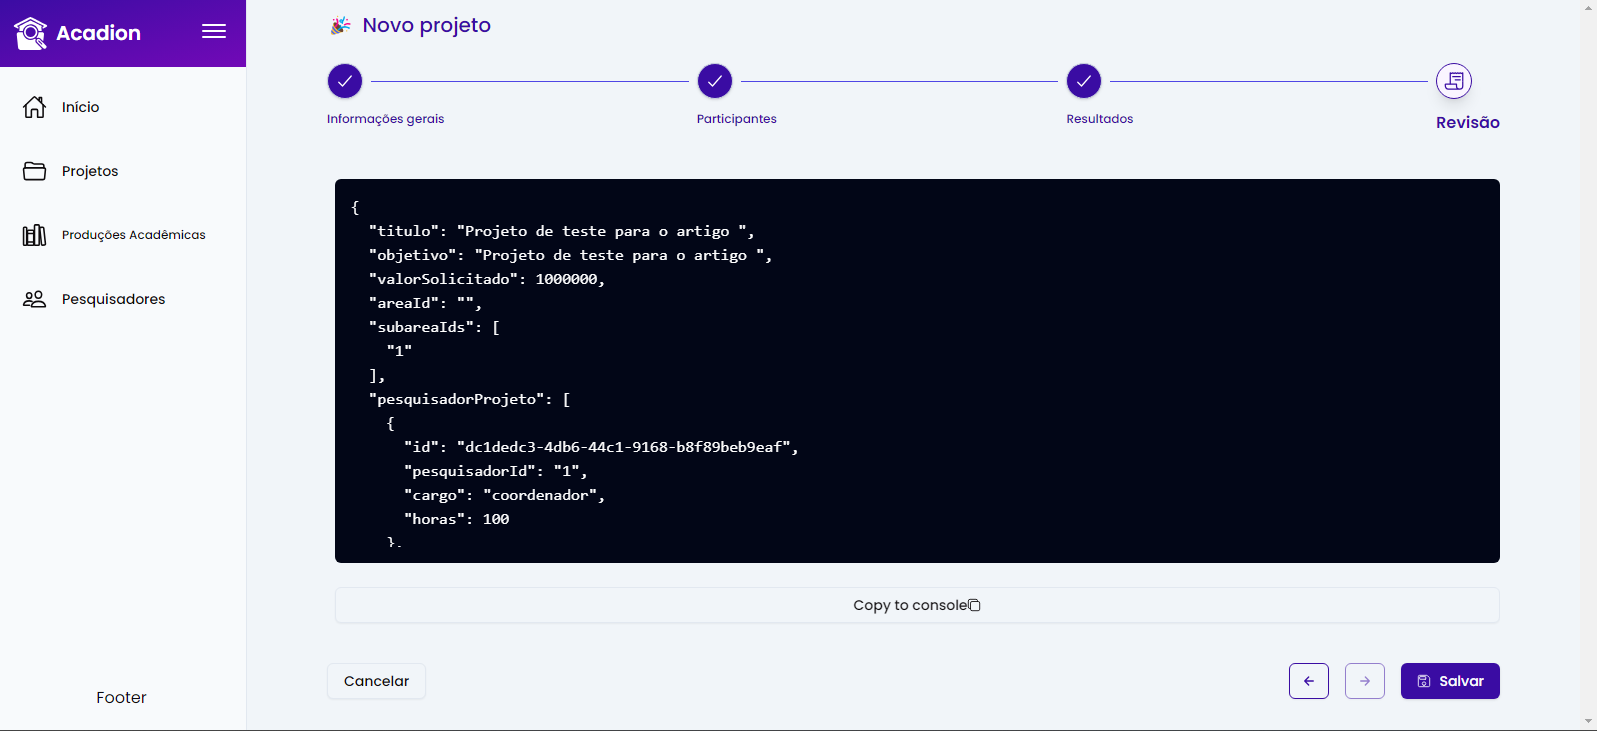
\includegraphics[width=1\linewidth]{figuras/NovoProjetoRevisao.png}
    \caption{Novo Projeto Revisão}
    \label{fig:enter-label}
\end{figure}

\begin{figure}[H]
    \centering
    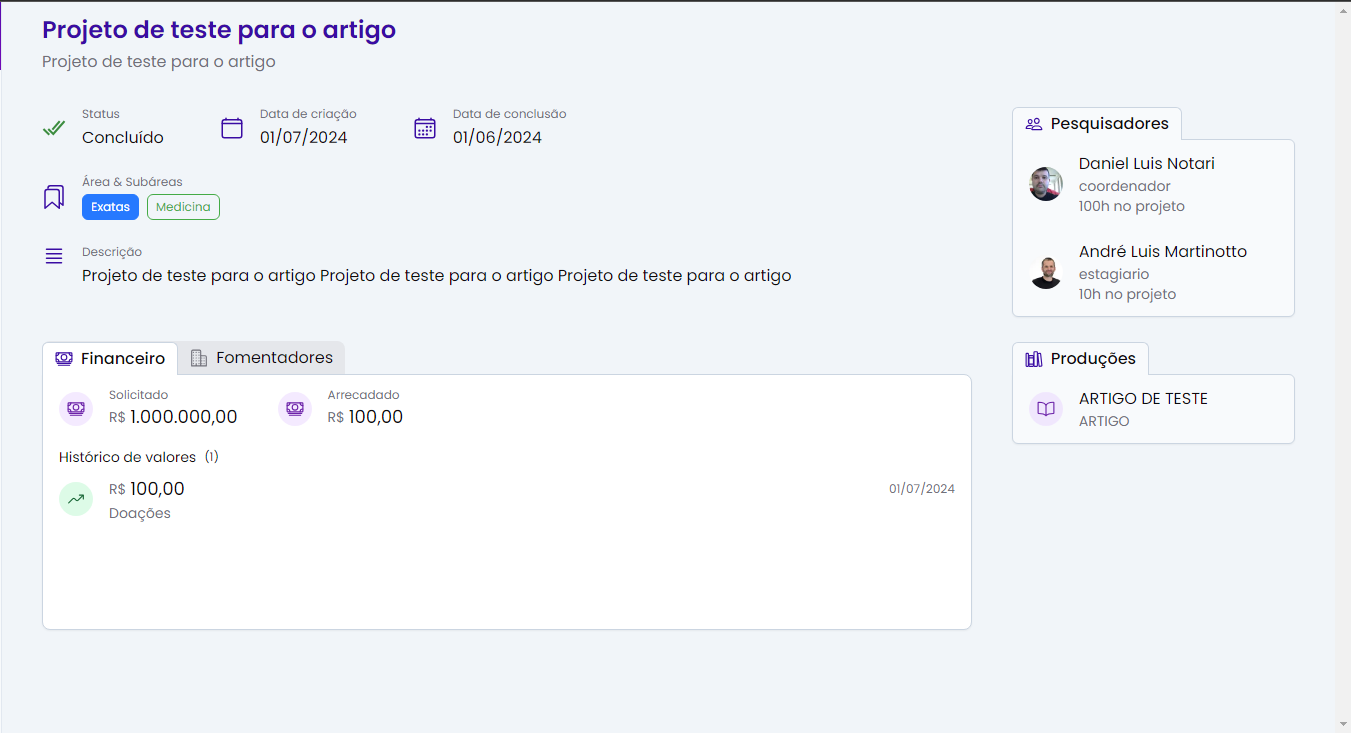
\includegraphics[width=1\linewidth]{figuras/NovoProjeto.png}
    \caption{Apos salvar o novo Projeto}
    \label{fig:newprojcreateweb}
\end{figure}

Após completar essas etapas das figuras \ref{fig:addnewprojweb} a \ref{fig:newprojcreateweb}, conseguimos salvar o projeto criado e adicioná-lo à lista de projetos.
\subsection{Acesso do Site}
URL: \hyperlink{https://acadion.vercel.app/}{https://acadion.vercel.app/}

\subsection{Observações da Implementação Web}
Algumas partes específicas da visualização de pesquisas ou de alguma produção acadêmica não foram implementadas nesta fase. No entanto, conseguimos criar e gerenciar projetos, incluindo suas publicações, dentro da aplicação web, dado o tempo disponível para a implementação.
Esta versão destaca o sucesso alcançado na implementação, enfatizando a fluidez e o design agradável obtidos. Para tornar o gerenciamento de dados viável, foi implementado um sistema rigoroso de validação no frontend.

\section{Implementação do Agente Desktop}

Durante o desenvolvimento do agente desktop, enfrentamos diversos desafios, tanto técnicos quanto conceituais. Um dos principais obstáculos foi aprender a linguagem Go (Golang), que foi escolhida pela sua eficiência e suporte nativo para concorrência. Além disso, foi necessário dominar o uso de \textit{Design Patterns} e implementar uma arquitetura \textit{N-tier} que atendesse aos requisitos de modularidade, escalabilidade e segurança do sistema.

Outro fator desafiador foi entender como implementar corretamente o agente para execução no sistema operacional Windows. Isso incluiu determinar a melhor forma de configurar o aplicativo para iniciar automaticamente com o sistema, sem interferir na experiência do usuário, e garantir que apenas uma instância do agente fosse executada por dispositivo.

A captação das informações foi outro ponto crítico. Era necessário que o agente coletasse dados como patrimônio, usuário logado e status do dispositivo, além de reportar essas informações de maneira eficiente e segura ao servidor. Implementar essa funcionalidade exigiu extensivas pesquisas e testes para garantir que o envio de dados fosse confiável e com baixo impacto no desempenho do sistema.

Além disso, trabalhamos na otimização do agente para operar de forma contínua sem causar sobrecarga no dispositivo ou na rede. Para isso, foram aplicados testes de desempenho e ajustes nos intervalos de coleta e envio de dados, garantindo um equilíbrio entre frequência de atualização e uso de recursos.

Embora desafiador, esse processo foi essencial para garantir que o agente desktop se integrasse perfeitamente ao restante do sistema, cumprindo seu papel de coletar e enviar informações em tempo real de maneira eficiente e segura.

\subsection{Arquitetura N-Tier do Agente}

A escolha pela Arquitetura \textit{N-Tier}, em vez de utilizar uma arquitetura em camadas convencional, como o \textit{Model-View-Controller} (MVC), foi motivada pelas especificidades do projeto de construção do agente. Diferentemente de sistemas web tradicionais, o agente desktop possui características e requisitos únicos, como a necessidade de comunicação direta e eficiente com o servidor, além da coleta e envio contínuos de dados.  

Dessa forma, optamos por projetar nossas próprias camadas, garantindo que cada parte do sistema estivesse alinhada às demandas do projeto e oferecendo maior flexibilidade para atender aos objetivos de desempenho, modularidade e escalabilidade.

\begin{figure}[H]
    \centering
    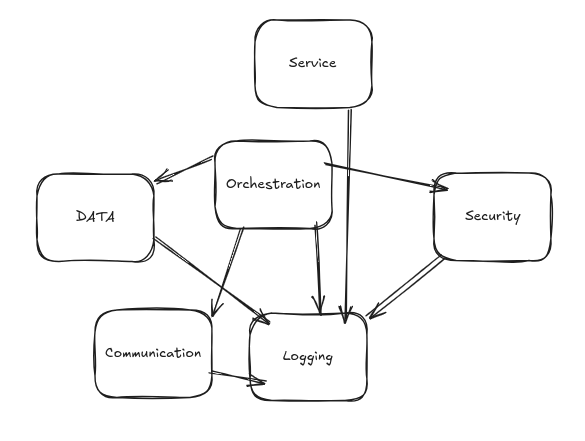
\includegraphics[width=1\linewidth]{figuras/NtierAgente.png}
    \caption{N-Tier Agente}
    \label{fig:NTagente}
\end{figure}

Na Figura: \ref{fig:NTagente} observamos o desenho das camadas que compõem a arquitetura do agente desktop. Cada camada possui responsabilidades bem definidas, conforme descrito abaixo:

\begin{itemize}
    \item \textbf{Service:} Responsável por criar e garantir que o agente seja executado como um serviço. Para isso, utilizamos a biblioteca \textit{Kardianos Service} em Golang, que facilita a configuração e o gerenciamento do serviço no sistema operacional.
    
    \item \textbf{Security:} Camada dedicada às funções de segurança. Atualmente, é responsável pela aplicação de HMAC nos \textit{JSONs}, garantindo a integridade e a autenticidade dos dados enviados ao servidor.
    
    \item \textbf{Logging:} Implementa um sistema de \textit{log} centralizado para capturar erros e informações relevantes da aplicação, permitindo o monitoramento eficiente e a depuração do sistema.
    
    \item \textbf{Data:} Camada encarregada da extração de informações do computador, como dados de hardware, IP, usuário logado e outras métricas relevantes.
    
    \item \textbf{Communication:} Cuida da comunicação com o \textit{back-end}, estabelecendo conexões seguras e confiáveis para enviar os dados coletados e receber respostas do servidor.
    
    \item \textbf{Orchestration:} A camada mais importante do agente, sendo responsável por integrar as demais camadas. Ela forma os \textit{JSONs}, aplica HMAC, coordena o envio para o servidor e organiza as funcionalidades para garantir o funcionamento harmonioso do sistema.
\end{itemize}
Em termos de autorização de comunicação entre as camadas, as seguintes regras foram definidas para garantir uma arquitetura modular e segura:

\begin{itemize}
    \item Todas as camadas têm permissão para acessar a camada \textbf{Logging}, permitindo o registro centralizado de erros e informações relevantes.
    \item A camada \textbf{Service} é isolada e não pode ser acessada por nenhuma outra camada, garantindo que sua funcionalidade seja protegida e executada apenas de forma controlada.
    \item A camada \textbf{Orchestration} possui permissões amplas, podendo acessar as camadas \textbf{Data}, \textbf{Communication}, \textbf{Security} e \textbf{Logging}. Isso reflete seu papel central na integração e coordenação das funcionalidades do agente.
\end{itemize}

Essa organização hierárquica das permissões reforça a modularidade do sistema, além de garantir que cada camada execute suas responsabilidades sem comprometer a segurança ou a integridade da aplicação.

\subsection{Design Patterns Utilizados no Agente}

De acordo com as diretrizes apresentadas por \textit{Refactoring Guru} (\url{https://refactoring.guru/design-patterns}), diversos \textit{Design Patterns} foram selecionados para a implementação do agente desktop, cada um atendendo a necessidades específicas do projeto. Os principais padrões aplicados foram:

\begin{itemize}
    \item \textbf{Singleton:} Utilizado para o objeto de \textit{Logging}, garantindo que apenas uma instância do sistema de registro de logs seja criada e utilizada por todo o programa, centralizando o controle e facilitando o monitoramento.

    \item \textbf{Factory:} Aplicado na criação de objetos responsáveis pela captura de informações do sistema, como dados de hardware e software. A \textit{Factory} verifica o sistema operacional (Windows ou Linux) e instancia os objetos apropriados para cada plataforma, garantindo flexibilidade e compatibilidade.

    \item \textbf{Builder:} Utilizado para a criação de \textit{JSONs}, permitindo construir de forma estruturada e modular as informações principais, como dados de \textit{Core}, programas instalados e especificações de hardware. Esse padrão facilita a adição de novos campos e melhora a manutenção do código.

    \item \textbf{Mediator:} Implementado na camada de \textit{Orchestration}, servindo como um intermediário para coordenar a comunicação e interação entre as diferentes camadas, como \textit{Data}, \textit{Security}, \textit{Communication} e \textit{Logging}.
\end{itemize}

A aplicação desses \textit{Design Patterns} foi essencial para garantir a modularidade, escalabilidade e organização do código, além de permitir um desenvolvimento mais eficiente e alinhado às melhores práticas de engenharia de software.

\subsection{Implementação do Agente}

Inicialmente, o agente foi planejado para funcionar em sistemas operacionais Linux e Windows. No entanto, devido ao curto prazo de implementação, optamos por focar no seu funcionamento exclusivamente em Windows. Apesar disso, grande parte do programa foi estruturada para permitir futuras adaptações para Linux, utilizando abordagens como o \textit{Factory Pattern}, que facilita a criação de objetos específicos para diferentes sistemas operacionais.

O agente é distribuído como um executável (\texttt{.exe}) que é executado em sistemas Windows 10 e 11. O processo de instalação ocorre da seguinte forma:

\begin{enumerate}
    \item No diretório \texttt{C:/}, crie uma pasta com um nome de sua preferência.
    \item Copie o arquivo \texttt{agente.exe} para dentro dessa pasta.
    \item Abra o \textit{Prompt de Comando} como administrador.
    \item Navegue até a pasta criada e execute o comando \texttt{./agente.exe install}.
\end{enumerate}

Após essa etapa, o agente cria um serviço no Windows chamado \textbf{LOTUS}, configurado para iniciar automaticamente. Esse serviço permite que o agente opere de forma contínua e integrada com o restante do sistema, garantindo a coleta e envio de dados de forma eficiente e transparente.

\subsection{Segurança do Agente}

Atualmente, a segurança do agente está parcialmente implementada, com destaque para o uso do HMAC (Hash-based Message Authentication Code). Essa funcionalidade foi integrada ao agente para garantir a integridade e autenticidade dos \textit{JSONs} enviados ao servidor. No entanto, o suporte correspondente no \textit{back-end} ainda não foi concluído, limitando sua aplicação prática no momento.

Outras medidas de segurança, como a implementação de um sistema de autenticação baseado em tokens e a troca de chaves para criptografia, foram planejadas, mas não foram priorizadas devido ao curto prazo de desenvolvimento. Embora ainda não implementadas, essas funcionalidades estão previstas para futuras atualizações do sistema, visando melhorar significativamente a proteção dos dados e das comunicações.

Apesar dessas limitações iniciais, a arquitetura do agente foi projetada para facilitar a inclusão dessas melhorias de segurança no futuro, garantindo que o sistema possa evoluir para atender a requisitos mais robustos.


\subsection{Informações Extras do Agente}

Futuramente, está planejada a criação de uma camada de configuração para o agente, utilizando arquivos no formato YAML. Essa camada permitirá configurar informações como rotas e outros parâmetros essenciais, visando simplificar a manutenção e personalização do agente conforme as necessidades específicas de cada ambiente.

Além disso, dentro da pasta onde o agente é configurado como serviço, serão gerados os seguintes arquivos:

\begin{itemize}
    \item \textbf{Arquivos de Log:} Criados automaticamente para registrar erros, eventos e informações relevantes do funcionamento do agente, facilitando a análise e depuração do sistema.
    \item \textbf{Arquivo \texttt{pat.txt}:} Esse arquivo armazena o patrimônio do computador, que é capturado a partir do nome da máquina. Caso o nome não contenha o número de patrimônio, será gerado automaticamente um número negativo aleatório como identificador.
\end{itemize}

Essas funcionalidades adicionais visam tornar o agente mais autossuficiente e adaptável, além de facilitar seu gerenciamento em ambientes distribuídos.
 



\section{Implementação do Back-end}
A aplicação adota o padrão MVC (Model-View-Controller), onde cada camada desempenha um papel fundamental na organização e funcionalidade do sistema. Na camada Model, localizada nos arquivos models.py, reside a estrutura de dados e a lógica de negócios, mapeando diretamente para tabelas do banco de dados. A camada View, implementada em views.py, cuida da apresentação e da lógica de controle, respondendo às chamadas de endpoints e processando dados para retorno apropriado. O Controller é gerenciado pelo Django por meio do URL dispatcher em urls.py, roteando requisições para as views corretas. Adicionalmente, Serializers são utilizados para converter modelos em instâncias JSON, facilitando a comunicação entre o backend e os clientes da API. Essa divisão estruturada não apenas organiza o código de maneira lógica, mas também promove escalabilidade e manutenção simplificada, permitindo o desenvolvimento e teste independentes de cada camada.

\subsection{Deploy do Back-end em nuvem}

Para o deployment da aplicação, optamos pelo serviço Cloud Run da Google Cloud Platform. Esse serviço oferece a flexibilidade necessária para executar containers de maneira escalável e automatizada. Inicialmente, configuramos um Dockerfile para definir o ambiente de execução da aplicação. Além disso, desenvolvemos scripts bash auxiliares que garantem a inicialização automática do servidor da aplicação ao iniciar o container, configurando a exposição da porta correta e outras configurações necessárias.

Adotamos também um webhook de integração contínua com o repositório GitHub. Esse webhook é configurado para acionar automaticamente o build de um novo container sempre que há um merge na branch principal do projeto. Essa prática assegura que o ambiente de produção esteja constantemente atualizado com as últimas alterações do código-fonte, minimizando a necessidade de intervenção manual e aumentando a eficiência do processo de deployment.

Para garantir a segurança e configurar variáveis de ambiente, utilizamos a interface intuitiva fornecida pelo console da Google Cloud Platform. Isso nos permitiu definir variáveis sensíveis de forma segura e aplicar configurações de segurança de tráfego diretamente na plataforma.
\section{Github para o Codigo Fonte}
https://github.com/Projetos-Faculdade-UCS/Projac

\section{Conclução da Implementação}
Em resumo, a implementação do backend foi um sucesso, com a aplicação sendo eficientemente hospedada na nuvem através do Google Cloud em containers Docker, oferecendo uma API robusta para ser consumida por aplicativos e servidores web. O aplicativo móvel foi completamente implementado, integrando todas as funcionalidades planejadas e proporcionando uma experiência de usuário completa. Embora o desenvolvimento da versão web não tenha sido concluído integralmente, conseguimos alcançar nossos objetivos principais, incluindo o cadastro de pesquisas e a apresentação de um design moderno e funcional.

\section{


































